\section{Problem Examples}
At present, our system includes seven CTF challenges, with one
disabled due to missing a key file. To give a sense of the style of
problems, and expected interactions with the problems, we will now
outline two different included challenges.

\subsection{Hitcon 2014's rsaha}
This challenge runs a small server encrypting messages using RSA. The server encrypts random messages and expects the plaintext as input. After succeffully decrypting 10 numbers, the server will give out the flag, which is of course also encrypted. As with many crypto CTF problems, the challenge uses a server primarily to limit the time to decrypt a messages. For each message, the user only has a window of 10 seconds to reply with the plaintext. This prevents any simple brute-force attacks.

The provided server source code shows how the messages are encrypted. The server uses naive RSA encryption without any padding. For each message, two random primes $p$ and $q$ with increasing bitlength between 50 and 450 bits are generated. The server computes the modulus $n=p\cdot q$ from it and encrypts the message with the public exponent $e=3$: $c_1\equiv m^3 \pmod{b}$. However, the server also returns $c_2\equiv (m+1)^3\pmod{b}$. 

But this allows us to use an attack published by Franklin and Reiter \cite{franklin1995linear}, which works if we have two messages $m_1$ and $m_2$ with $m_1 +1 = m_2$ and three as the public exponent:

\[ \frac{c_2+2c_1-1}{c_2-c_1+2} = \ldots \]

\subsection{PlaidCTF 2014's parlor}

\begin{figure}[!ht]
\centering
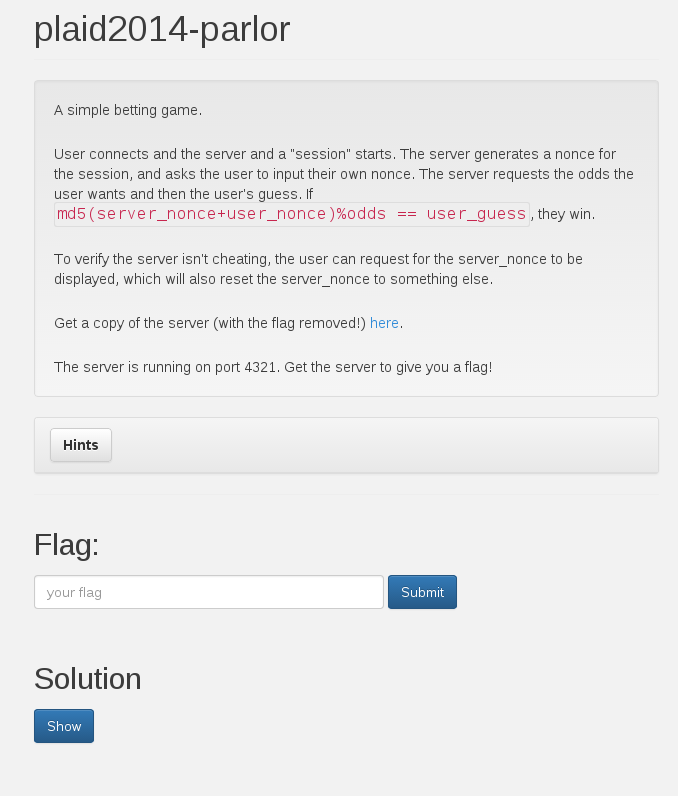
\includegraphics[width=0.5\textwidth]{parlor_page.png}
\caption{Plaid2014 parlor challenge page}\label{fig:parlor_page}
\end{figure}

\begin{figure}[!ht]
\centering
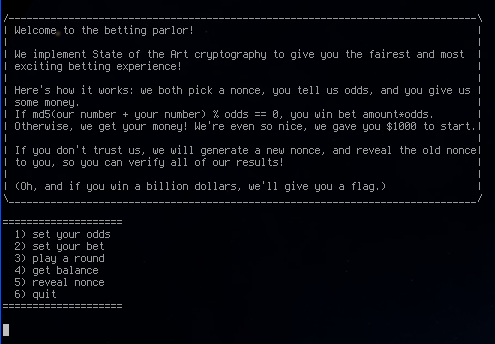
\includegraphics[width=0.5\textwidth]{parlor_interface.png}
\caption{Plaid2014 parlor server text-based interface}\label{fig:parlor_interface}
\end{figure}


This challenge is a small server that runs a betting game. The game
lets you set 'odds' (the minimum number of $0$ bits at the end of the
md5sum that causes a win), and submit a player nonce value,
\texttt{pnonce}.  The server then generates an md5sum as
\texttt{md5(snonce+pnonce)} where \texttt{snonce} is a nonce supplied
by the server. While the player must submit a new unique
\texttt{pnonce} for each bet, the server will re-use \texttt{snonce}
until the player requests to see it for verification purposes. To
facilitate proving the honest of the server, it sends back the lower
100 bits of the md5sum after each bet. This means that after some
series of bets, the player can request to see the (now old)
\texttt{snonce} and verify that the 100 bit sequences they got match
the md5sums generated by \texttt{md5(snonce+pnonce)}.

This setup, however, still leaves the server vulnerable to a
\textit{hash-length extension} attack. In the classic form, the
attacker is able to generate any sum they wish, given something of the
form \texttt{md5(snonce+pnonce)} where they know the resulting md5sum
and \texttt{pnonce}. This can be achieved using tools like
\texttt{hashpump}, which are explicitly designed to implement this
attack. However, in this case, the attacker has additional
restrictions. First, they do not know \texttt{snonce} OR the first 28
bits of any md5sum from the server. Second, they must win multiple
times, and cannot send the same \texttt{pnonce} more than once.

To solve this, the attacker simply bruteforces the first 28 bits of
the md5sum of some known \texttt{md5(snonce+pnonce)}. This can be done
by asking the server for \texttt{md5(snonce+pnonce)} and
\texttt{md5(snonce+pnonce+L)}, then trying to do a hash-length
extension with $L$ on all possible versions of the first (28 bits of
brute force) to see if they match the result. This will result in a
solution for the FULL 128 bits of \texttt{md5(snonce+pnonce)}. Now a
standard hash-length extension attack targeting a result ending in all
0 bits can be done.\cite{parlor:mslc}

After running the attack, and submitting a series of \texttt{pnonce}
values that always result in ending 0 bits, the attacker has a large
amount of money and the server happily hands over a flag.

This problem represents a very standard CTF problem design; a basic
server (just a single python file) that plays a game that cannot be
won fairly. Our design makes integrating problems like this very
simple. Filling out the description and hints is straight forward,
but the suggested reading had to be careful not to only include
links to hash-length extension attacks. The server configuration is
mostly handled by the templated init script that the new problem
generation tool uses. The problem designer needs only fill out two
lines of a configuration file (with the problem name and server
binary), and write any description and solution information they wish
to include.

Figure \ref{fig:parlor_page} shows the rendered page generated by our
scripts for this problem. After connecting to the server on the port
specified (via \texttt{nc localhost 4321}) they are presented with the
problem interface as designed by the challenge author (see Figure
\ref{fig:parlor_interface}.) This is a standard looking CTF challenge,
with a basic text-based server interface.
